\graphicspath{{fig/sim_studies/}}

\chapter{Simulation studies}
\label{cha:sim_studies}

The feasibility of performing parameter inference on real data can be assessed
by simulation study. In simulation studies, candidate models are forward
simulated for \emph{known} parameter values. This simulated data is then used
to assess whether the known parameter values can be captured by inference.

Simulation studies provide good opportunity to assess (and frankly, debug) our
implementation of MCMC algorithms constructed to sample realisations from the
posterior distribution. If a simulation study is successful, then the
statistical machinery built to perform the inference on simulated data can be
repurposed to perform inference on \emph{real} data. If parameter inference is
\emph{not} possible on simulated data, we know that the same inference will not
be possible on real data either.

\section{Global models}
\label{sec:global_models}

Global models refer to models in which all agents take the \emph{same}
parameter values. These are in contrast to hierarchical models, in which all
agents take \emph{different} parameter values. We shall first seek to perform
simulation studies on these global models, as they represent a simpler
inference problem.

Recall from Bayes' Theorem (\cref{eq:bayes_theorem}) that to realise the
posterior distribution we need to combine the likelihood of the data with our
prior beliefs. Let us begin by considering the likelihood of observing a single
agent updating its direction, in the presence of neighbours, from $\theta_{i,
t}$ to $\theta_{i, t+1}$. From \cref{eq:students_update} we have that agent $i$
updates its direction as a draw from the generalised Students $t$-distribution
with location $\angmean{\theta}_{i,t}$, scale $\sigma_Y$ and degrees of freedom
$\nu$. As such, the likelihood of observing this directional update can be
quantified by the probability density of the generalised Student's $t$
distribution with $\nu$ degrees of freedom, location $\angmean{\theta}_{i,t}$,
and scale $\sigma_Y$, evaluated at $\theta_{i,t+1}$:
\begin{equation*}
  L(\sigma_Y, \nu, \angmean{\theta}_{i,t} \given \theta_{i,t+1}) =
  \frac{\Gamma(\frac{\nu +1 }{2})}{\Gamma(\frac{\nu}{2})\sqrt{\pi\nu}\sigma_Y}
  \Bigg(1 + \frac{1}{\nu}
  \bigg(\frac{\theta_{i,t+1}-\angmean{\theta}_{i,t}}{\sigma_Y}\bigg)^2
  \Bigg)^{-\frac{\nu+1}{2}},
\end{equation*}
where $\Gamma$ is the gamma function. Building on this, let us consider the
likelihood of observing agent $i$'s directional updates from time $t$ to time
$t+2$. As the noise experienced by an agent is independent between time steps,
we may express this likelihood as the product:
\begin{align*}
  L(\sigma_Y,\nu,\angmean{\theta}_{i,t},\angmean{\theta}_{i,t+1}\given\theta_{i,t+1},
  \theta_{i,t+2})
  = L(\sigma_Y,\nu,\angmean{\theta}_{i,t+1}\given\theta_{i,t+2})\times
  L(\sigma_Y,\nu,\angmean{\theta}_{i,t}\given\theta_{i,t+1}).
\end{align*}

In general, we wish to express the likelihood of observing agent $i$'s
directional updates over any number of times steps. Suppose then that we
observe the directions of agent $i$ from time $t=1$ to time $t=T$. Again, as
consecutive realisations from the noise distribution are independent, we can
compute the likelihood as a product
\begin{align*}
  L(\sigma_Y, \nu, \angmean{\theta}_{i,1:T-1} \given \theta_{i,2:T})
  = & \prod_{t=1}^{T-1} L(\sigma_Y,\nu,\angmean{\theta}_{i,t} \given \theta_{i,t+1}) \\
  = & \prod_{t=1}^{T-1}
  \frac{\Gamma(\frac{\nu +1 }{2})}{\Gamma(\frac{\nu}{2})\sqrt{\pi\nu}\sigma_Y}
  \Bigg(1 + \frac{1}{\nu}
  \bigg(\frac{\theta_{i,t+1}-\angmean{\theta}_{i,t}}{\sigma_Y}\bigg)^2
  \Bigg)^{-\frac{\nu+1}{2}},
\end{align*}
where $\angmean{\theta}_{i,1:T-1}$ is shorthand for
$\angmean{\theta}_{i,1},\angmean{\theta}_{i,2},\ldots,\angmean{\theta}_{i,T-1}$,
and similarly for $\theta_{i,2:T}$. Finally, although we have expressed the
likelihood of observing a single agent's directional changes over $T$
observations, we really wish to express the likelihood of observing \emph{an
entire flock's} directional changes over $T$ observations. Consider observing a
flock of $N$ individuals over $T$ time steps. The likelihood of observing their
directional updates can be quantified as:
\begin{align}
  \label{eq:likelihood}
  \begin{split}
    L(\sigma_Y, \nu, \angmean{\theta}_{1:N,1:T-1} \given\theta_{1:N,2:T})
    &= \prod_{i=1}^N \prod_{t=1}^{T-1} L(\sigma_Y,\nu,\angmean{\theta}_{i,t}\given\theta_{i,t+1})  \\
    &= \prod_{i=1}^N \prod_{t=1}^{T-1}
    \frac{\Gamma(\frac{\nu +1 }{2})}{\Gamma(\frac{\nu}{2})\sqrt{\pi\nu}\sigma_Y}
    \Bigg(1 + \frac{1}{\nu}
    \bigg(\frac{\theta_{i,t+1}-\angmean{\theta}_{i,t}}{\sigma_Y}\bigg)^2
    \Bigg)^{-\frac{\nu+1}{2}}.
  \end{split}
\end{align}

The likelihood function for all our models takes the same form. What differs
between models is the specification of the weighting function $\omega_{ij,t}$
and the corresponding computation of $\angmean{\theta}_{i,t}$.

\subsection{Vicsek model}
\label{ssec:vicsek_sim_study}

We simulate the Vicsek model to realise a flock of $N=45$ agents moving for
$T=200$ time steps. We desire to work with simulated data which is similar to
real data (see, for example,
\cref{fig:seq_1_traj,fig:seq_2_traj,fig:seq_3_traj}). As such, the initial
conditions for this simulation are taken from an observation of a real flocking
event, to be introduced in the proceeding chapter: \cref{cha:sheep}. Parameters
$r=50$, $\sigma_Y=0.03$ and $\nu=7$ are set for this simulation.
\cref{fig:vicsek_sim} shows the data generated by this simulation. We seek to
assess whether we can recover the true parameter values from the simulated
data.

\begin{figure}[tbp]
  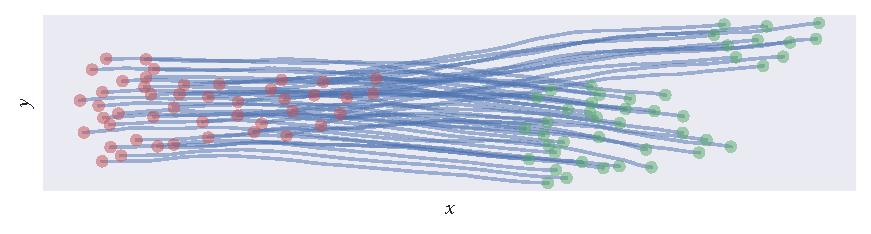
\includegraphics{r/r_sim.pdf}
  \caption{The trajectories of $N=45$ agents simulated over $T=200$ time steps
      according to the Vicsek model. The initial conditions of the simulation
      reflect that of a real flocking event, introduced in the proceeding
      \cref{cha:sheep}. The parameters of the model are given by $r=50$,
      $\sigma_Y=0.03$ and $\nu=7$. Initial conditions and parameter values were
      chosen with the intention to generate a simulated flock similar to that
      of a real flocking event. At $t=0$ agents are positioned at the locations
      represented by the green markers. Agents travel along the blue lines, with
      the red markers representing their positions at the end of the simulation.}
  \label{fig:vicsek_sim}
\end{figure}

The likelihood of observing the data can be quantified by \cref{eq:likelihood}.
However, to target the posterior we also need to specify our prior beliefs
about the model parameters. To allow the data to drive the inference, we shall
specify weakly informative priors. Once realisations from the posterior have
been made, we overlay our priors to assess how our beliefs have updated in
light of the data.

Our prior beliefs about likely values for the degrees of freedom parameter
$\nu$ shall be reflected by a $\Ga(2, 0.1)$ distribution, as popularised by
\textcite{juarez10}. As $r$ and $\sigma_Y$ both represent strictly positive
measures, we shall use a gamma distribution to quantify our beliefs about them.
These prior beliefs, as detailed in \cref{eq:vicsek_priors} and visualised in
\cref{fig:vicsek_priors}, represent vague beliefs, allowing a large range of
possible parameter values.
\begin{align}
  \label{eq:vicsek_priors}
  \begin{split}
    r           & \sim \Ga(50, 1) \\
    \sigma_Y    & \sim \Ga(2, 100)\\
    \nu         & \sim \Ga(2, 0.1)
  \end{split}
\end{align}
\begin{figure}[tbp]
  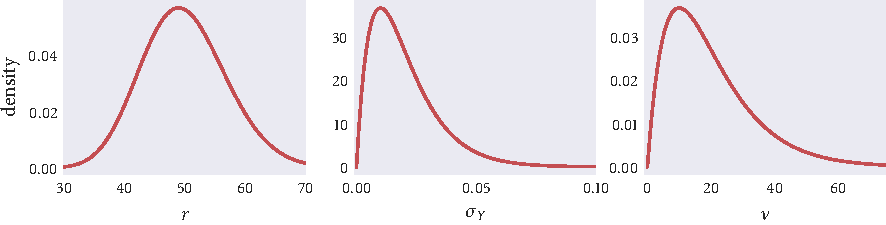
\includegraphics{r_priors.pdf}
  \caption{Probability density functions representing our prior beliefs about
      plausible parameter values of the Vicsek model. These distributions
      represent weakly-informative priors, allowing a large range of possible
      parameter values. These beliefs are expressed mathematically in
  \cref{eq:vicsek_priors}.}
  \label{fig:vicsek_priors}
\end{figure}

Having specified the likelihood function, and quantified our prior beliefs
about the model parameters, we now have all the ingredients necessary to target
the posterior. Unfortunately, the discontinuity in the weighting function of
the Vicsek model results in a discontinuous posterior. As Stan (the
probabilistic programming language introduced in \cref{ssec:hmc}) requires a
continuous-parameter valued posterior that is differentiable almost everywhere,
we are unable to use Stan and instead target the posterior distribution with a
random walk Metropolis--Hastings sampler.

We implement the random walk sampler for 1,100,000 iterations. The first
100,000 iterations of the scheme are discarded to allow the sampler to
converge. The chains were initialised as draws from our prior beliefs. The
output of this scheme is summarised in
\cref{tab:vicsek_summary}.

\cref{fig:vicsek_trace} shows the chains generated by our inference scheme,
having discarded the initial burn-in period. From these trajectories we see
evidence that our sampler has converged: the chains oscillating around fixed
locations with some common variance. The samples generated by these chains are
visualised in \cref{fig:vicsek_hist}. The true parameter values used to
generate the simulated data are shown by vertical green lines. See that in each
posterior the true value is successfully captured by the posterior density, and
lies close to the posterior mode. The posterior densities about the parameters
$\nu$ and $\sigma_Y$ look Gaussian, however, the posterior distribution over
$r$ is non-Gaussian. The non-Gaussian form of the posterior about $r$ is a
product of the discontinuous interaction rule which it represents. Our prior
beliefs are overlain in red and appear flat in comparison to our posteriors,
reflecting that our beliefs have updated considerably in light of the data.

\begin{table}[p]
  \begin{tabular}{@{}crrrrr@{}}
    \toprule
    Parameter    & mean  & sd   & 5\%   & 95\%  & ESS     \\
    \midrule
    $r$          & 50.02 & 0.04 & 49.99 & 50.11 & 12\,290 \\
    $\sigma_{Y}$ & 0.03  & 0.00 & 0.03  & 0.03  & 44\,560 \\
    $\nu$        & 7.01  & 0.51 & 6.31  & 7.99  & 47\,420 \\
    \bottomrule
  \end{tabular}
  \caption{Summarising the posterior realisations for the parameters inferred
    in fitting the Vicsek model to simulated data. Realisations were made by
    implementing a random walk Metropolis--Hastings sampler. Columns report
    the posterior mean and standard deviation for each parameter. In addition
    to this, the fifth and ninety-fifth percentiles of our posteriors are
    quantified. Finally, the effective sample size (ESS) of each chain is
    computed (and rounded to the nearest multiple of ten). The large values
    of the ESS observed give reliability to our computed posterior summaries.}
  \label{tab:vicsek_summary}
\end{table}%
\begin{figure}[p]
  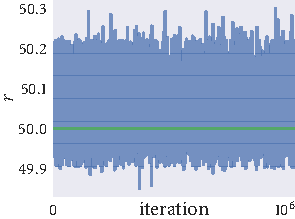
\includegraphics{r/r_trace_r.pdf}%
  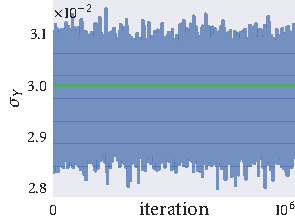
\includegraphics{r/r_trace_sigma_Y.pdf}%
  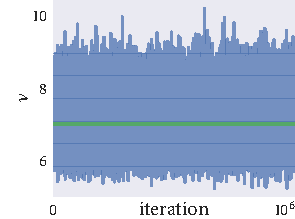
\includegraphics{r/r_trace_nu.pdf}
  \caption{Sequences generated by a random-walk Metropolis--Hastings algorithm
    fitting the Vicsek model to simulated data. The initial 100,000
    iterations are discarded to allow a burn-in period. Horizontal green
    lines represent the true parameter values used to generate the simulated
    data. The chains look well-behaved, showing no irregularities, and suggest
    that our sampler has converged.}
  \label{fig:vicsek_trace}
\end{figure}%
\begin{figure}[p]
  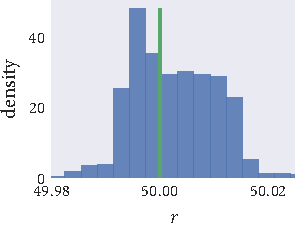
\includegraphics{r/r_hist_r.pdf}%
  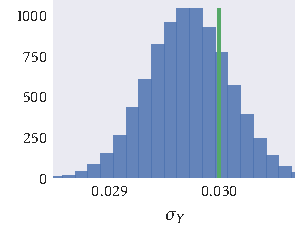
\includegraphics{r/r_hist_sigma_Y.pdf}%
  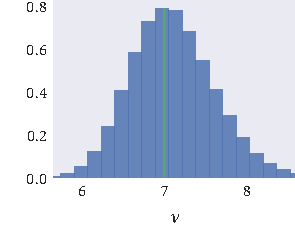
\includegraphics{r/r_hist_nu.pdf}
  \caption{Distributions of the posterior samples drawn in fitting the Vicsek
      model to simulated data. The green lines represent the known parameter
      values which we seek to recover. Prior beliefs are overlain in red. Our
      posterior densities are seen to accurately capture the true parameter
      values. The data can be seen to have been very informative, as our
      posterior densities have updated considerably from our prior beliefs.}
  \label{fig:vicsek_hist}
\end{figure}

Considering the output of this simulation study, we conclude that we can
accurately infer the true parameter values of data simulated from the Vicsek
model. This gives us confidence in moving forward to fit this model to real
data.

\subsection{Continuous models}
\label{ssec:continuous_models}

We have demonstrated that we can fit the Vicsek model to simulated data. We
now seek to fit the power-law weighted (\cref{eq:power_law_interaction}) and
Gaussian weighted (\cref{eq:gaussian_interaction}) models to simulated data.

As these models implement continuous interaction rules, we may attempt
parameter inference using the Stan programming language. \cref{eq:likelihood}
can be used to quantify the likelihood of observing simulated data. To target
the posterior we combine this likelihood with our prior beliefs.

The power-law and Gaussian weighted models represent similar interaction rules.
As with the parameters $\nu$, $\sigma_Y$ and $r$, we shall use gamma
distributions to quantify our prior beliefs about $\alpha$ and $\sigma_X$. To
ensure that our prior beliefs between these models are consistent, we shall
determine our beliefs by considering plausible values of the weighting
$\omega_{ij,t}$. Using information about $d_{ij,t}$, along with
\cref{eq:power_law_interaction,eq:gaussian_interaction}, we can use our beliefs
about $\omega_{ij,t}$ to derive beliefs about $\alpha$ and $\sigma_X$.

To realise our prior beliefs we shall make two probabilistic statements about
$\omega_{ij,t}$. These can be used to determine prior distributions which best
reflect these statements. Firstly, we consider the weighting which agent $i$
gives to its closest neighbour at time $t$. We believe with probability 0.025
that this weighting will be less than or equal to 0.25. Similarly, we believe
with probability 0.975 that the weighting which agent $i$ gives to its fifth
closest neighbour will be less than or equal to 0.90. More concisely, we can
express these statements as:
\begin{align}
  \label{eq:omega_statements}
  \begin{split}
    P(\omega_{ij, t}({\min_j(d_{ij,t}, 1)}) \leq 0.25) & = 0.025, \\
    P(\omega_{ij, t}({\min_j(d_{ij,t}, 5)}) \leq 0.90) & = 0.975,
  \end{split}
\end{align}
where $\omega_{ij, t}({\min_j(d_{ij,t}, k)})$ is the influence of agent $i$'s
$k$-th closest neighbour at time $t$. To determine prior beliefs which best
reflect these statements, we seek shape and scale parameters for our gamma
priors which minimise:
\begin{equation*}
  [P(\omega_{ij, t}({\min_j(d_{ij,t}, 1)}) \leq 0.25) - 0.025]^2
  + [P(\omega_{ij, t}({\min_j(d_{ij,t}, 5)}) \leq 0.90) - 0.975]^2.
\end{equation*}
A simple numerical optimisation routine can be used to minimise this function.
With this we realise prior beliefs:
\begin{align}
  \label{eq:gauss_power_priors}
  \begin{split}
    \alpha   & \sim \Ga(2, 2) \\
    \sigma_X & \sim \Ga(5, 5),
  \end{split}
\end{align}
which we visualise in \cref{fig:gauss_power_priors}.

\begin{figure}[tbp]
  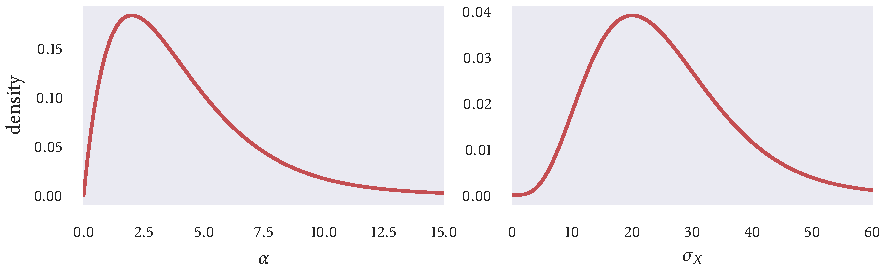
\includegraphics{gauss_power_priors.pdf}
  \caption{Probability density functions representing our prior beliefs about
    $\alpha$ and $\sigma_X$, the interaction parameters of the power-law and
    Gaussian weighted models respectively. These prior beliefs are given
    analytically in \cref{eq:gauss_power_priors}. Our prior beliefs about
    these interaction parameters represent equivalent beliefs about the
    weighting function $\omega_{ij,t}$.}
  \label{fig:gauss_power_priors}
\end{figure}

\subsubsection{Power-law weighted}
\label{sssec:power_law_sim_study}

The initial conditions for our simulated data are taken from an observation of
a real flocking event, the same event used to initialise the simulation in
\cref{ssec:vicsek_sim_study}. A realistic-looking flock is generated with
parameters $\alpha=1.5$, $\sigma_Y=0.03$ and $\nu=7$
(\cref{eq:power_law_interaction}). \cref{fig:power_sim} shows the trajectories
realised by this simulation. We then seek to recover the known parameter values
by inference.
\begin{figure}[tbp]
  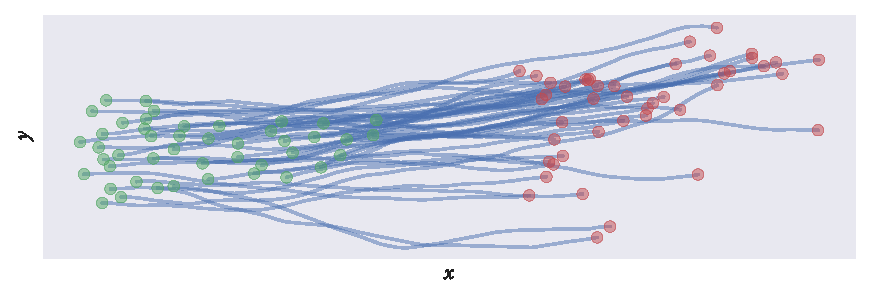
\includegraphics{power/power_sim.pdf}
  \caption{Simulated data generated by a run of the power-law weighted model
    with parameter values $\alpha=1.5$, $\sigma_Y=0.03$ and $\nu=7$. The data
    represents the trajectories of motion of $N=45$ agents moving for $T=200$
    frames. Initial conditions for this simulation were realised from an
    observation of a real flocking event.}
  \label{fig:power_sim}
\end{figure}

Stan is used to perform parameter inference on this model. Four independent
chains are initialised as realisations from our prior beliefs. Each chain is
then simulated for 10,000 iterations, with the first 5000 iterations discarded
to allow a warm-up period. \cref{tab:power_summary} summarises the posterior
draws generated by this run. The tabulated split-$\widehat{R}$ values
(\cref{eq:rhat}) indicate that our sampler has converged for all parameter
values.

\begin{table}[tbp]
  \begin{tabular}{@{}crrrrrr@{}}
    \toprule
    Parameter    & mean & sd   & 5\%  & 95\% & ESS     & $\widehat{R}$ \\
    \midrule
    $\alpha$     & 1.50 & 0.02 & 1.48 & 1.54 & 13\,130 & 1.0           \\
    $\sigma_{Y}$ & 0.03 & 0.00 & 0.03 & 0.03 & 11\,400 & 1.0           \\
    $\nu$        & 7.09 & 0.50 & 6.28 & 7.91 & 11\,580 & 1.0           \\
    \bottomrule
  \end{tabular}
  \caption{Summarising the posterior realisations made by Stan fitting
    simulated data to the power-law weighted model. Columns show the
    posterior mean and standard deviation of each model parameter, along with
    the fifth and ninety-fifth percentiles of our beliefs. The number of
    effective samples drawn from the posterior is quantified by the ESS. The
    values of $\widehat{R}$ computed indicate that our chains have all
    converged.}
  \label{tab:power_summary}
\end{table}

The chains generated by this sampler are shown in \cref{fig:power_trace}. Each
colour represents an independent chain. Although the four chains were
initialised at different locations, they all converge to the same region.

\begin{figure}[tbp]
  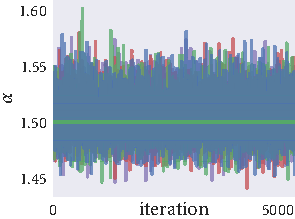
\includegraphics{power/power_trace_alpha.pdf}%
  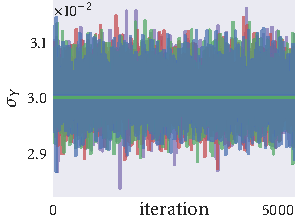
\includegraphics{power/power_trace_sigma_Y.pdf}%
  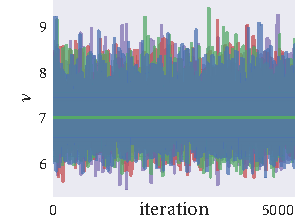
\includegraphics{power/power_trace_nu.pdf}
  \caption{Trajectories of the four independent chains for each parameter
    inferred in fitting the power-law weighted model to simulated data. Each
    independent chain is overlain in a different colour. Although each chain
    was initialised at a different starting point, they can be seen to
    converge to the same distribution. Chains were simulated for 10,000
    iterations, with the first 5000 iterations discarded to allow
    convergence. The chains appear well-behaved, showing no irregularities
    and are seen to oscillate around the true parameter values, represented
    by the green horizontal lines.}
  \label{fig:power_trace}
\end{figure}

Histograms of our posterior draws are presented in \cref{fig:power_hist}. The
vertical green lines in these plots represent the true parameter values. In
each case, our posteriors can be seen to capture the true values. In fact, the
true parameter values are seen to be well represented by the posterior mode. In
contrast with the posteriors derived in fitting the Vicsek model to simulated
data (\cref{ssec:vicsek_sim_study}), the posterior distribution of the
interaction parameter (here $\alpha$), \emph{is} Gaussian. Recall that our
posterior density about $r$ (\cref{fig:vicsek_hist}) was non-Gaussian, owing to
the discontinuous weighting rule it represents. Our prior beliefs are overlain
in red. These priors appear flat in comparison to our posteriors, indicating
that we have learnt a lot from the data.

\begin{figure}[tbp]
  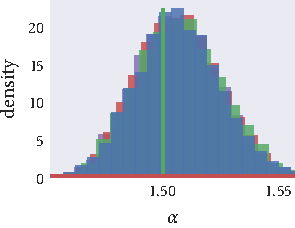
\includegraphics{power/power_hist_alpha.pdf}%
  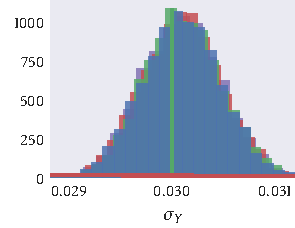
\includegraphics{power/power_hist_sigma_Y.pdf}%
  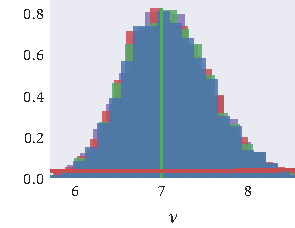
\includegraphics{power/power_hist_nu.pdf}
  \caption{Histogram plots of our samples drawn from the posterior distribution
    in fitting simulated data to the power-law weighted model. The true
    parameter values are represented by the green vertical lines. See that
    the true value for each parameter is well represented by the posterior
    mode. Prior beliefs are overlain in red, and appear flat in comparison to
    our posterior densities. This indicates that the observed data was
    informative, and that our prior beliefs did not adversely effect our
    posterior densities.}
  \label{fig:power_hist}
\end{figure}

\subsubsection{Gaussian weighted}

As with the previous simulation studies, we forward simulate this model with
$N=45$ agents and $T=200$ time steps, using the same initial state used in
\cref{ssec:vicsek_sim_study,sssec:power_law_sim_study}. \cref{fig:gauss_sim}
illustrates the data generated by this simulation. Here, parameters
$\sigma_X=20$, $\sigma_Y=0.025$ and $\nu=7$ were used to produce
realistic-looking flocking behaviour.

\begin{figure}[tbp]
  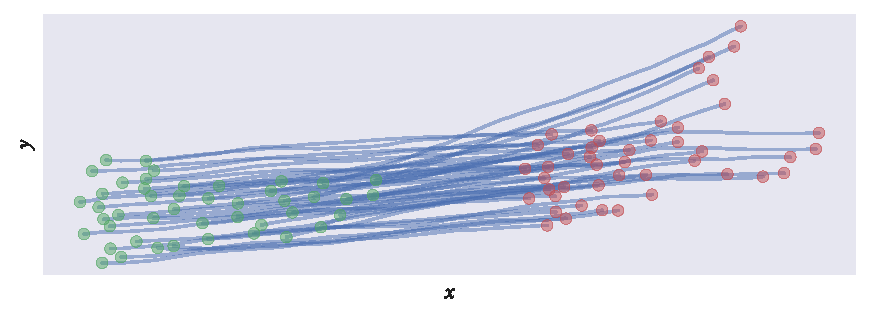
\includegraphics{gauss/gauss_sim.pdf}
  \caption{Data generated from a simulation of the Gaussian weighted model with
    parameters $\sigma_X=20$, $\sigma_Y=0.025$ and $\nu=7$. A total of $N=45$
    agents were simulated for $T=200$ time steps. Initial conditions
    were taken from an observation of a real flocking event, with the intention
    to generate data similar to that of an observed flock.}
  \label{fig:gauss_sim}
\end{figure}

We shall use Stan to perform parameter inference. Four independent sequences
are initialised at draws from our prior beliefs and simulated for 10,000
iterations. The first 5000 iterations are discarded to allow for a warm-up
period. \cref{tab:gauss_summary} summarises the output from this run. The
reported split-$\widehat{R}$ values indicate that the sequences have converged.

The output visualised in \cref{fig:gauss_trace,fig:gauss_hist} shows a
well-behaved sampler, capable of capturing the true parameter values of the
Gaussian weighted model from simulated data.

\begin{table}[tbp]
  \begin{tabular}{@{}crrrrrr@{}}
    \toprule
    Parameter    & mean  & sd   & 5\%   & 95\%  & ESS     & $\widehat{R}$ \\
    \midrule
    $\sigma_{X}$ & 19.94 & 0.20 & 19.60 & 20.27 & 13\,310 & 1.0           \\
    $\sigma_{Y}$ & 0.025 & 0.00 & 0.024 & 0.025 & 11\,700 & 1.0           \\
    $\nu$        & 7.25  & 0.53 & 6.41  & 8.12  & 11\,360 & 1.0           \\
    \bottomrule
  \end{tabular}
  \caption{Summaries of the posterior densities realised in fitting the
    Gaussian weighted model to simulated data. Each row represents a
    parameter of the Gaussian model. Each column presents a different summary
    of our posterior density. The computed $\widehat{R}$ indicate that the
    simulated chains converged, and the realised ESS values show a
    satisfactory number of draws made from the posterior.}
  \label{tab:gauss_summary}
\end{table}%
\begin{figure}[tbp]
  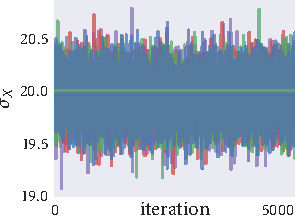
\includegraphics{gauss/gauss_trace_sigma_X.pdf}%
  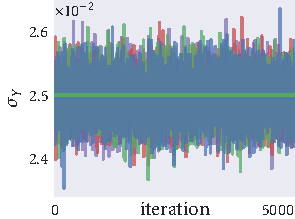
\includegraphics{gauss/gauss_trace_sigma_Y.pdf}%
  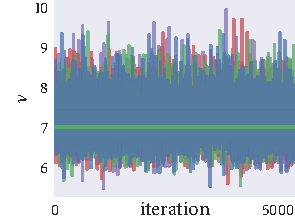
\includegraphics{gauss/gauss_trace_nu.pdf}
  \caption{Visualising the Markov chains generated fitting the Gaussian
    weighted model to simulated data. Each colour chain represents an independent
    chain. Although the chains are initialised as different draws from our
    priors, they all converge to the same common distribution. The chains look
    well-behaved; they show no irregularities, and are observed to oscillate
    around the true parameter values with constant variance.}
  \label{fig:gauss_trace}
\end{figure}%
\begin{figure}[tbp]
  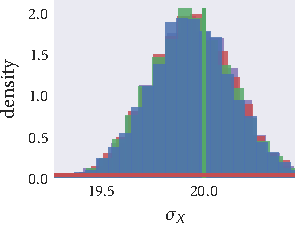
\includegraphics{gauss/gauss_hist_sigma_X.pdf}%
  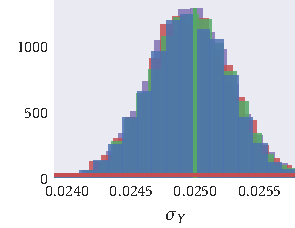
\includegraphics{gauss/gauss_hist_sigma_Y.pdf}%
  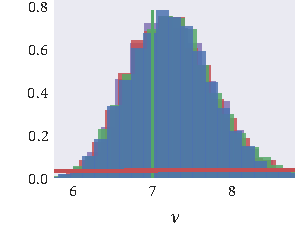
\includegraphics{gauss/gauss_hist_nu.pdf}
  \caption{Draws realised by Stan in fitting the Gaussian weighted model to
    simulated data. The true values (green vertical lines) are well
    represented by the posterior mode. Our posteriors appear much more peaked
    than our priors (overlain in red), suggesting that our choice of priors
    had little influence over the realised posteriors.}
  \label{fig:gauss_hist}
\end{figure}

\subsection{Topological model}

In \cref{ssec:continuous_models} we demonstrated that it is possible to
accurately capture the parameters of the power-law and Gaussian weighted models
from simulated data. However, we are interested in comparing the
predictive-performance of metric and topological models with real data. As
such, we need a simulation study on our topological model.

\cref{eq:likelihood,eq:top_interaction} allow us to quantify the goodness of
fit of the topological model with parameters $k$, $\sigma_Y$ and $\nu$ to
observations of a flocking event. To target the posterior we must combine this
likelihood with prior beliefs about the model parameters. We have no reason to
believe that the noise experienced by individuals under a topological regime
would be any different to that experienced under a metric regime. As such, our
prior beliefs about the noise parameters $\sigma_Y$ and $\nu$ shall remain the
same as in the metric case: as expressed in \cref{eq:vicsek_priors}.

We are then left to quantify our prior beliefs about $k$, the number of nearest
neighbours which an agent interacts with. Previous work suggested that agents
interact with their six to seven nearest neighbours \parencite{ballerini08}.
However, this work investigated three-dimensional flocking events of flying
birds. As we are focusing on data restricted to a two-dimensional
plane---flocking sheep (\cref{cha:sheep}) and swimming birds
(\cref{sec:scoters})---we believe that the number of nearest neighbours will be
lower than the six to seven found previously. We find that a $\Ga(6, 1/2)$
distribution captures a wide range of plausible values for $k$
(\cref{fig:top_priors}).

\begin{figure}[tbp]
  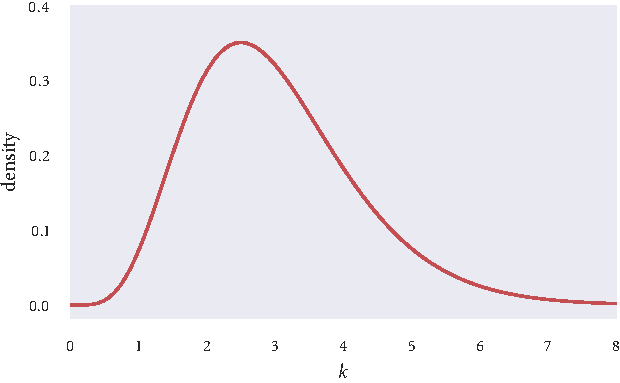
\includegraphics{top/top_priors.pdf}
  \caption{Prior beliefs about the number of nearest neighbours $k$ which an
  agent interacts with in a $2$-dimensional environment, expressed by a $\Ga(6,
  1/2)$ distribution. Our prior beliefs here are in part informed by the work
  of \textcite{ballerini08}.}
  \label{fig:top_priors}
\end{figure}

The topological model is forward simulated to generate data for the simulation
study. Forty-five agents are simulated for two-hundred time steps. Each agent
interacts with its closest $k=3$ nearest neighbours. Noise was generated from a
generalised Student's $t$-distribution with scale $\sigma_Y=0.03$ and degrees
of freedom $\nu=7$. The trajectories generated by this simulation are
illustrated in \cref{fig:top_sim}, and resemble that of a real flocking event.

\begin{figure}[tbp]
  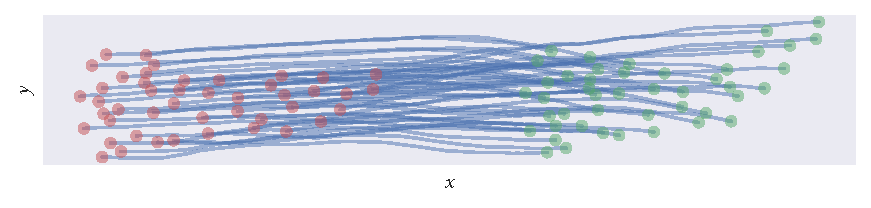
\includegraphics{top/top_sim.pdf}
  \caption{Data used for our simulation study of the topological model. Each
    agent was simulated to interact with its nearest $k=3$ neighbours, and was
    subject to noise generated from a generalised Student's $t$-distribution
    with location $\mu=0$, scale $\sigma_Y=0.03$ and degrees of freedom $\nu=7$.}
  \label{fig:top_sim}
\end{figure}
\begin{table}[tbp]
  \begin{tabular}{@{}crrrrrr@{}}
    \toprule
    Parameter    & mean & sd   & 5\%  & 95\% & ESS     & $\widehat{R}$ \\
    \midrule
    $k$          & 2.98 & 0.02 & 2.94 & 3.02 & 16\,710 & 1.0           \\
    $\sigma_{Y}$ & 0.03 & 0.0  & 0.03 & 0.03 & 13\,240 & 1.0           \\
    $\nu$        & 7.04 & 0.50 & 6.20 & 7.81 & 13\,355 & 1.0           \\
    \bottomrule
  \end{tabular}
  \caption{Tabulating summaries of the posterior draws made in fitting the
    topological model to simulated data. Posterior samples were generated by
    Stan's implementation of the No-U-Turn-Sampler. Each row represents a
    parameter of the topological model. The values of ESS and $\widehat{R}$
    computed show that the chains converged and realised a large number of
    posterior samples.}
  \label{tab:top_summary}
\end{table}
\begin{figure}[tbp]
  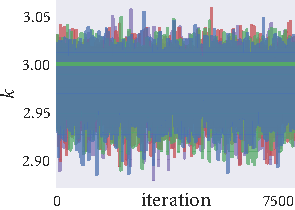
\includegraphics{top/top_trace_k.pdf}%
  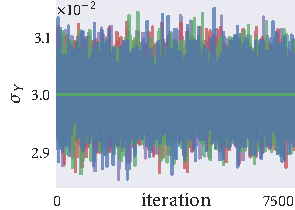
\includegraphics{top/top_trace_sigma_Y.pdf}%
  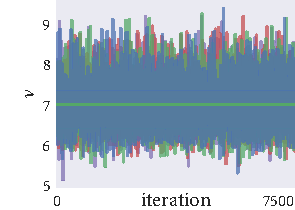
\includegraphics{top/top_trace_nu.pdf}
  \caption{Markov chains generated in inferring the parameters of the
    topological model from simulated data. Stan was used to simulate four
    independent chains constructed to target the posterior distribution.
    These chains were initialised at different initial conditions. The
    resulting chains are seen to converge to the same common distribution, and
    oscillate regularly around the true parameter values.}
  \label{fig:top_trace}
\end{figure}
\begin{figure}[tbp]
  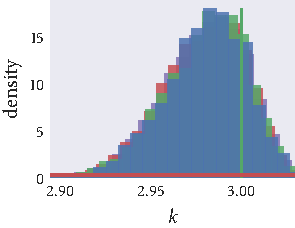
\includegraphics{top/top_hist_k.pdf}%
  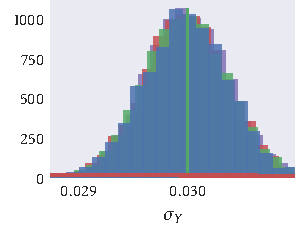
\includegraphics{top/top_hist_sigma_Y.pdf}%
  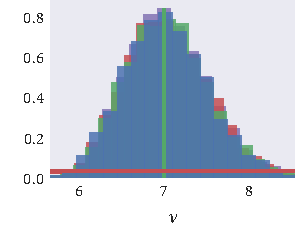
\includegraphics{top/top_hist_nu.pdf}
  \caption{Histogram plots of our posterior densities having fitted the
    topological model to simulated data. Our posteriors are seen to have
    updated considerably from our prior beliefs (overlain in red), and accurately
    capture the true values (green vertical lines).}
  \label{fig:top_hist}
\end{figure}

Stan was used to make realisations from the posterior distribution. Four
independent chains were initialised at draws from our prior beliefs. Each chain
was simulated for 10,000 iterations. The initial 2500 iterations were
discarded to allow the chains to converge. The sequences generated by this
sampler are shown in \cref{fig:top_trace}. Corresponding posteriors are
plotted in \cref{fig:top_hist}. Our prior beliefs about the model parameters
are overlain in red, and appear flat in comparison to our posteriors:
indicating that we have learnt a lot in observing the data. Summaries of this
output are tabulated in \cref{tab:top_summary}. Considering the output of this
scheme we see that we can accurately recover the true parameter values of data
simulated from the topological model.

\section{Hierarchical models}
\label{sec:hier_mod_studies}

Hierarchical models represent a more demanding inference problem owing to the
increased number of model parameters to infer. The simulation studies performed
in \cref{sec:global_models} required three parameters to be inferred per model:
one interaction parameter and two noise parameters (scale and degrees of
freedom). In the hierarchical models introduced in \cref{ssec:hier_mod} each
agent has its \emph{own} interaction parameter, as well as its \emph{own} scale
parameter for the noise distribution. For simplicity, the agents share a global
degrees of freedom parameter for the noise distribution. To fit a hierarchical
model to data describing the movements of $N$ individuals we are then required
to infer $2N+1$ parameters and $4$ hyperparameters.

Introducing this extra level of structure into our model needs to be accounted
for in the likelihood function. The likelihood function for our differing
hierarchical models takes the same general form. For illustration purposes,
here we shall consider the likelihood of data generated from a hierarchical
Gaussian weighted model. The likelihood function for the remaining hierarchical
models can be derived in a similar fashion.

Suppose we simulate the movements of $i=1,\ldots,N$ individuals over
$t=1,\ldots,T$ time steps, according to a hierarchical Gaussian weighted model.
Here, agent $i$ has interaction parameter $\sigma_{X_i}$ and noise-scale
parameter $\sigma_{Y_i}$. The interaction parameters are distributed according
to a population-level distribution, here taking the form of a gamma
distribution with mean $m_X$ and variance $v_X$ (\cref{eq:sigma_X_hierarchy}).
Noise-scale parameters $\sigma_{Y_i}$ are distributed in a similar manner
(\cref{eq:sigma_Y_hierarchy}). The likelihood of observing this flock's
directional updates, along with the parameters $\sigma_{X_i}$ and
$\sigma_{Y_i}$ can be expressed as the product:
\begin{align}
  \label{eq:hier_likelihood}
  \begin{split}
      L(\sigma_X, \sigma_Y, \nu, \angmean{\theta}_{1:N,1:T-1} &\given \theta_{1:N,2:T},
    m_X, v_X, m_Y, v_Y) \\
    &= L(\sigma_Y, \nu, \angmean{\theta}_{1:N,1:T-1} \given \theta_{1:N,2:T}) \times
    L(m_X, v_X \given \sigma_X)
    \times
    L(m_Y, v_Y \given \sigma_Y).
  \end{split}
\end{align}
Taking the form of the likelihood from \cref{eq:likelihood} and considering the
hierarchy imposed in \cref{eq:sigma_Y_hierarchy,eq:sigma_X_hierarchy}, we may
write down the likelihood in full as:
\begin{align}
  \begin{split}
      L(\sigma_X, \sigma_Y, \nu, \angmean{\theta}_{1:N,1:T-1} \given \theta_{1:N,2:T}&,
    m_X, v_X, m_Y, v_Y) \\
    &= \prod_{i=1}^N \prod_{t=1}^{T-1}
    \frac{\Gamma(\frac{\nu +1 }{2})}{\Gamma(\frac{\nu}{2})\sqrt{\pi\nu}\sigma_Y}
    \Bigg(1 + \frac{1}{\nu}
    \bigg(\frac{\theta_{i,t+1}-\angmean{\theta}_{i,t}}{\sigma_Y}\bigg)^2
    \Bigg)^{-\frac{\nu+1}{2}}\\
    &\hphantom{=}\times\prod_{i=1}^N \frac{(m_X / v_X)^{m_X^2 / v_X}}{\Gamma(m_X^2/v_X)}
        \sigma_{X_i}^{m_X^2/v_X - 1} \exp\bigg(-\frac{m_X}{v_X}\sigma_{X_i}\bigg)\\
    &\hphantom{=}\times\prod_{i=1}^N \frac{(m_Y / v_Y)^{m_Y^2 / v_Y}}{\Gamma(m_Y^2/v_Y)}
        \sigma_{Y_i}^{m_Y^2/v_Y - 1} \exp\bigg(-\frac{m_Y}{v_Y}\sigma_{Y_i}\bigg).\\
  \end{split}
\end{align}

\subsection{Continuous models}

In \cref{ssec:continuous_models} we used Stan to perform parameter inference on
data simulated from continuous models, and a random-walk Metropolis--Hastings
algorithm to perform inference on the Vicsek model. Similarly, here we shall
use Stan to perform parameter inference on data simulated from our
\emph{hierarchical} continuous models. However, owing to the increase in
dimensionality of the problem, performing inference on the hierarchical Vicsek
model with a Metropolis--Hastings algorithm (necessary because of the
discontinuous posterior) was found to be computationally infeasible, and is
omitted from this study.

\subsubsection{Power-law weighted}

\cref{fig:power_hier_sim} shows data simulated from the hierarchical power-law
weighted model. The interaction parameters of the 45 simulated agents are
drawn from a gamma distribution with mean $m_{\alpha}=1.2$ and variance
$v_{\alpha}=0.02$. The noise-scale parameters of the agents are drawn from a
gamma distribution with mean $m_Y=0.04$ and variance $v_Y=0.001$. As such,
$m_{\alpha}$, $v_{\alpha}$, $m_Y$ and $v_Y$ represent the hyperparameters of
this model.

\begin{figure}[tbp]
  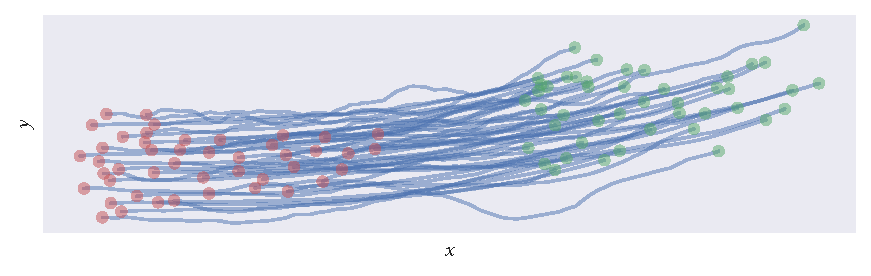
\includegraphics{power/power_hier_sim.pdf}
  \caption{Forward simulation of the hierarchical power-law weighted model. The
    movements of $N=45$ agents are simulated for $T=200$ time steps. For
    realism, the initial positions and directions of motions of the agents
    are taken from an observation of a real flocking event. The interaction
    parameters $\alpha_i$ are drawn from a gamma distribution with mean
    $m_{\alpha}=1.2$ and variance $v_{\alpha}=0.02$. Similarly, the
    noise-scale parameters $\sigma_{Y_i}$ are realisations from a gamma
    distribution with mean $m_Y=0.04$ and variance $v_Y=0.001$.}
  \label{fig:power_hier_sim}
\end{figure}

Vague hyperpriors are chosen to represent our prior beliefs about the
hyperparameters. These, along with the likelihood function, are combined with
Bayes' Theorem to target the posterior distribution. We use Stan's NUTS
algorithm to simulate four independent chains to target the posterior. Each
chain is initialised as a draw from our prior beliefs and simulated for 5000
iterations. The initial 2500 iterations are discarded to allow the chains to
converge from their initial conditions toward the posterior.

Our posterior realisations of the hyperparameters are visualised in
\cref{fig:power_hier_hist}. Each coloured histogram overlain represents the
realisations generated by an independent chain. Our hyperpriors are overlain in
red. See that in all cases our hyperpriors appear flat in comparison to our
posteriors. This reflects having updated our beliefs considerably in light of
the data. In this plot vertical green lines represent \emph{population}-level
summary statistics (the true values of the hyperparameters), and the vertical
black lines represent the corresponding \emph{sample}-level summary statistics.
For example, consider that although the $\alpha_i$ were drawn from a
distribution with population mean $m_{\alpha}=1.20$ (vertical green line),
their sample mean was $\overline{\alpha}\approx1.18$ (vertical black line). We
see that all the hyperparameters are well-captured by our posterior
distributions, and conclude that they can be accurately inferred from simulated
data.

\begin{figure}[tbp]
  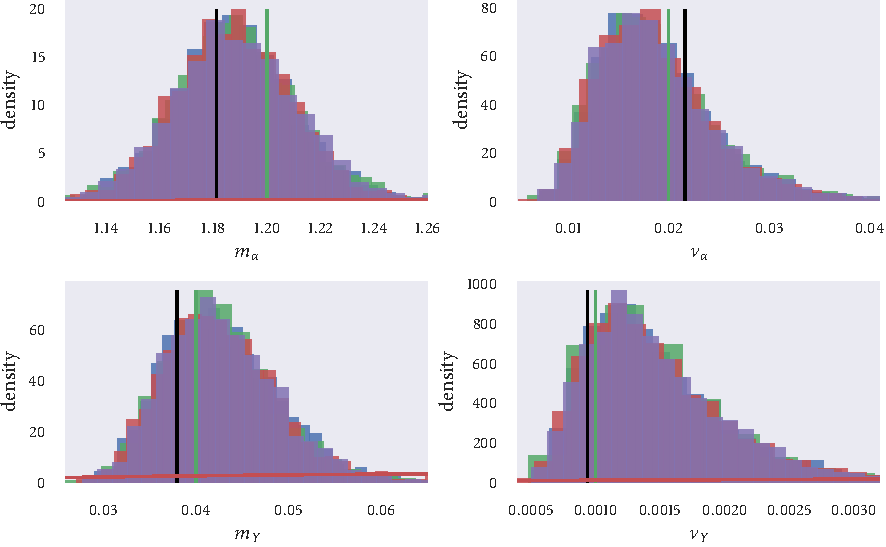
\includegraphics{power/power_hier_hist.pdf}
  \caption{Histogram plots representing our posterior densities about the
    hyperparameters of the hierarchical power-law weighted model fitted to
    simulated data. Vertical green lines represent the true values of the
    hyperparameters (the \emph{population} means and variances of the
    parameters). Vertical black lines represent \emph{sample} means and
    variances of the parameters. Hyperpriors are overlain in red.}
  \label{fig:power_hier_hist}
\end{figure}

Posterior densities about the $N$ interaction and $N$ noise-scale parameters are
summarised in \cref{fig:power_hier_summary}. Here, each boxplot represents a
posterior density. As is convention, box boundaries represent the $25$th and
$75$th percentiles of the posterior. Whiskers represent the median
$\pm1.5\times\text{IQR}$. See that in all but one case ($\alpha_6$), the true
parameter values lie within our posteriors. We observe that the
$\sigma_{Y_i}$'s are generally well represented by the posterior median. It
appears that smaller noise-scale parameters can be captured with less
uncertainty than larger noise-scale parameters. Although forty-four of the
forty-five interaction parameters are captured by our posteriors, the
interaction parameters are not recovered with as much accuracy as the
noise-scale parameters. However, we still see that our posteriors generally
capture the interaction parameters. 

\begin{figure}[tbp]
  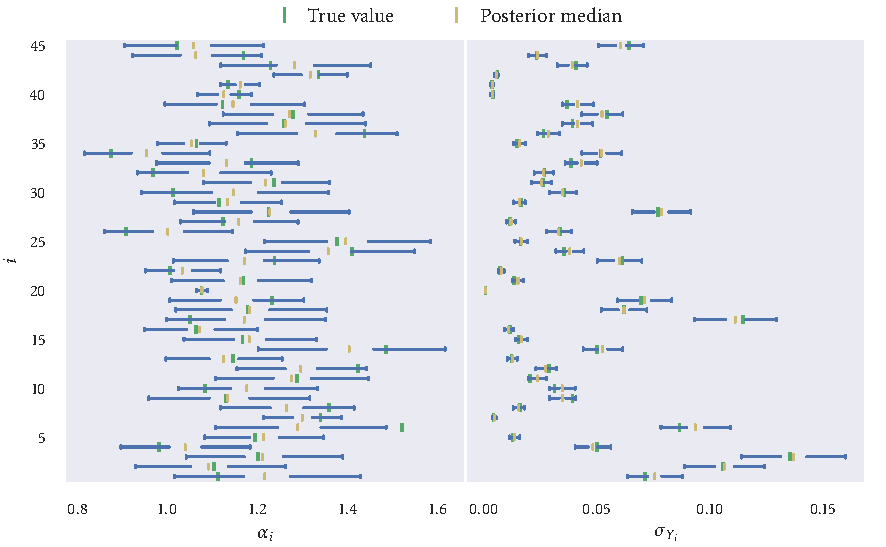
\includegraphics{power/power_hier_summary.pdf}
  \caption{Boxplots summarising our posteriors about the interaction and
    noise-scale parameters of the hierarchical power-law weighted model
    fitted to simulated data. As is convention, boxes show the $25$th, $50$th
    (the median) and $75$th percentiles of the posterior. Whiskers represent
    the median $\pm 1.5\times\text{IQR}$.}
  \label{fig:power_hier_summary}
\end{figure}

Although not included here for brevity, tabulating split-$\widehat{R}$ for
every parameter reveals that all chains converged with
$\widehat{R}=1.00$. Computing the effective sample size for each
parameter showed that the \emph{worst} performing chain still realised
approximately 10,000 effective samples from the posterior. This gives
confidence that our posteriors have been well realised.

Considering the posterior samples generated by our Stan model, we have
demonstrated that we can accurately recover the hyperparameters and parameters
of data simulated from a hierarchical power-law weighted model.

\subsubsection{Gaussian weighted}

In a similar manner to the simulation study just performed on the hierarchical
power-law weighted model, we now seek to perform a simulation study on the
hierarchical Gaussian weighted model. As before, our model is implemented to
simulate the movements of 45 agents over 200 observations. Here, the
interaction parameters $\sigma_{X_i}$ are drawn randomly from a gamma
distribution with mean $m_X=25$ and variance $v_X=1$. The forty-five
$\sigma_{X_i}$'s sampled for this simulation have mean
$\overline{\sigma_X}\approx25.2$ and variance $\text{Var}(\sigma_X)\approx1.1$.
The trajectories realised by this simulation are illustrated in
\cref{fig:gauss_hier_sim}.

\begin{figure}[tbp]
  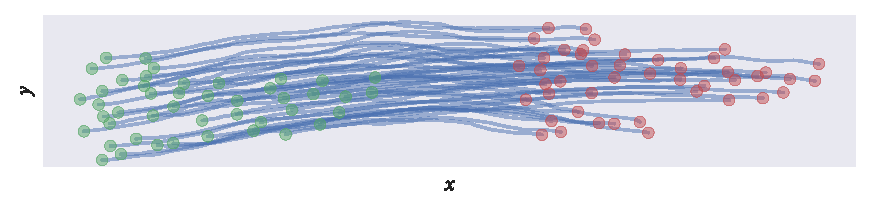
\includegraphics{gauss/gauss_hier_sim.pdf}
  \caption{Data generated by a simulation of the hierarchical Gaussian weighted
    model. The interaction parameters $\sigma_{X_i}$ are sampled from a gamma
    distribution with mean $m_X=25$ and variance $v_X=1$. Similarly, the
    noise-scale parameters are drawn from a gamma distribution with mean
    $m_Y=0.04$ and variance $v_Y=0.001$.} 
  \label{fig:gauss_hier_sim}
\end{figure}

We use the Stan modelling language to codify \cref{eq:hier_likelihood} and
express our vague prior beliefs about the hyperparameters of the model. Four
independent chains are again simulated for 5000 iterations, with the first
2500 iterations discarded to allow a warm up period.

Our posterior realisations about the hyperparameters are visualised in
\cref{fig:gauss_hier_hist}. The four independent chains simulated are seen to
have converged to a common distribution. The true values of the hyperparameters
(vertical green lines) lie well within our posteriors, and lie close to
the posterior mode.

\begin{figure}[tbp]
  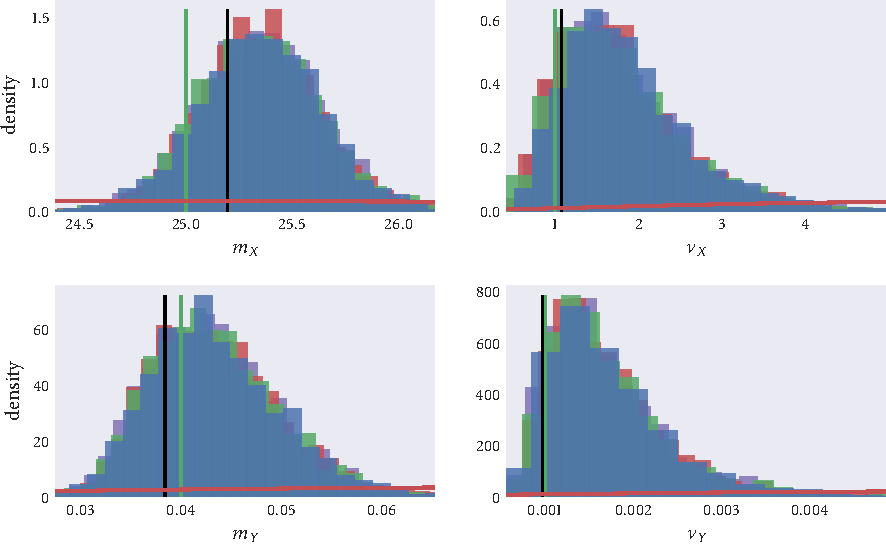
\includegraphics{gauss/gauss_hier_hist.pdf}
  \caption{Realisations from the posterior distribution of the hierarchical
    Gaussian weighted model. Vertical green lines show the true values of the
    hyperparameters. Vertical black lines show the sample summary statistics
    of the model parameters. Hyperpriors are overlain in red.}
  \label{fig:gauss_hier_hist}
\end{figure}

\cref{fig:gauss_hier_summary} is constructed to provide a convenient summary of
our posterior distributions about the $2\times N = 90$ model parameters used
for this simulation. The true parameter values are shown by green markers, and
posterior medians are represented by yellow markers. All the true parameter
values are seen to lie within our posteriors, indicating that they can
be captured by parameter inference. Our posteriors about the interaction
parameters of the agents overlap considerably. This indicates that the
parameters drawn for simulation represent very similar interaction weightings.
The noise-scale parameters, on the other hand, are captured with much less
uncertainty and overlap.

\begin{figure}[tbp]
  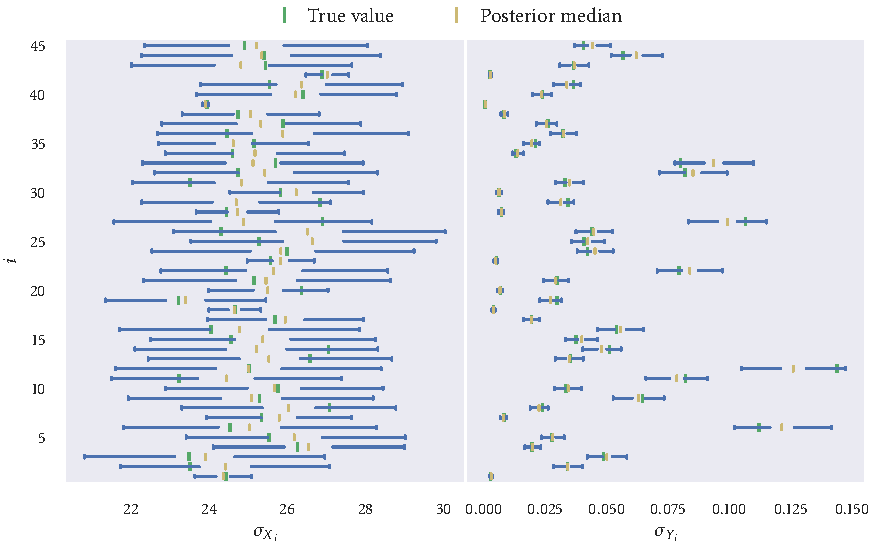
\includegraphics{gauss/gauss_hier_summary.pdf}
  \caption{Boxplots summarising the posterior densities about the interaction
    parameters and the noise-scale parameters used to forward simulate the
    hierarchical Gaussian weighted model. Each boxplot illustrates the
    posterior median, lower and upper quartiles, and the posterior median
    $\pm1.5\times\text{IQR}$.}
  \label{fig:gauss_hier_summary}
\end{figure}

\subsection{Topological model}

Having satisfied ourselves that we can fit continuous hierarchical models to
simulated data, we now turn our attention to our hierarchical topological
model. The data simulated for this study is shown by the trajectories of
\cref{fig:top_hier_sim}. The trajectories generated for this simulation bear a
strong resemblance to that of a real flocking event (see, eg.
\cref{fig:seq_1_traj}).

\begin{figure}[tbp]
  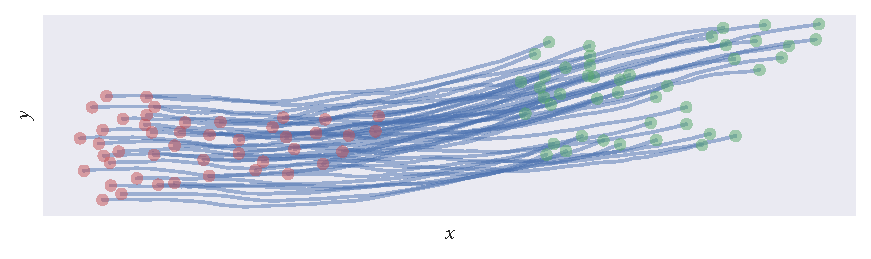
\includegraphics{top/top_hier_sim.pdf}
  \caption{An illustration of the trajectories realised by a forward
    simulation of the hierarchical topological model. In this model agent $i$
    interacts with its $k_i$ nearest neighbours, and experiences noise
    distributed according to a Student's $t$-distribution with scale
    $\sigma_{Y_i}$ and degrees of freedom $\nu$. Interaction and noise scale
    parameters are drawn from population level distributions, parameterised by the
    hyperparameters $m_k=1$, $v_k=2$, $m_Y=0.4$ and $v_Y=0.001$.}
  \label{fig:top_hier_sim}
\end{figure}

Interaction and noise-scale parameters were drawn from population-level
distributions. The interaction parameters $k$ were sampled from a Gamma
distribution with mean $m_k=4$ and variance $v_k=2$. These hyperparameters are
represented in \cref{fig:top_hier_hist} by vertical green lines. The sampled
interaction parameters had mean $\overline{k}\approx4.15$, and variance
$\text{Var}(k)\approx1.25$. These values are illustrated in
\cref{fig:top_hier_hist} with vertical black lines. In a similar manner, the
noise-scale parameters are drawn from a Gamma distribution with hyperparameters
$m_Y=0.4$ and $v_Y=0.001$, which resulted in parameters $\sigma_Y$ with sample
mean $\overline{\sigma_Y}\approx0.035$ and sample variance
$\text{Var}(\sigma_Y)\approx0.001$.

The posterior samples realised by Stan's implementation of the
No-U-Turn-Sampler are shown in \cref{fig:top_hier_hist}. These histograms
represent the posterior realisations made by four independent Markov chains,
each simulated for 5000 iterations and initialised at different locations.
Sample and population level summary statistics of the parameters are shown to
be captured well by our posterior densities, indicating that we can
successfully recover the hyperparameters of simulated data by inference. Our
posteriors are much more peaked than our hyperpriors, suggesting that our
choice of hyperprior had little influence over our posteriors, as was intended.

\begin{figure}[tbp]
  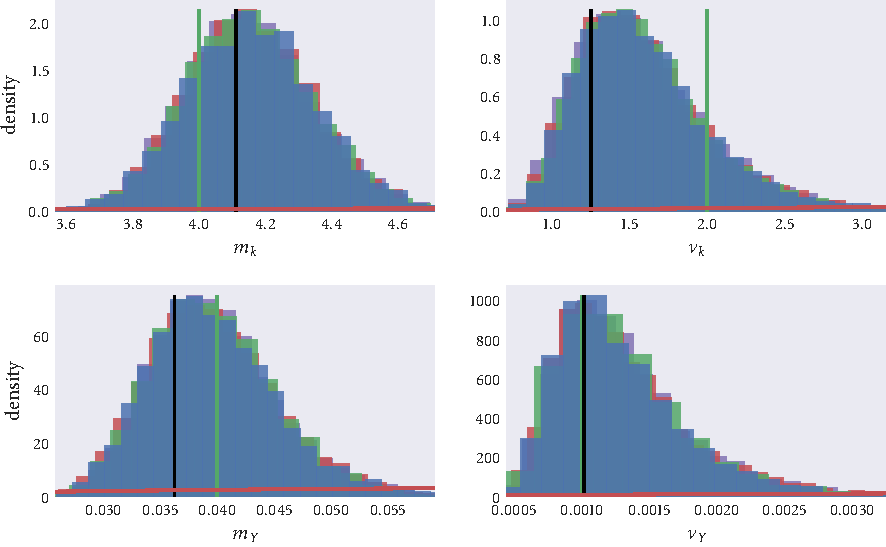
\includegraphics{top/top_hier_hist.pdf}
  \caption{Histogram plots showing the posterior samples drawn in fitting the
    hierarchical topological model to simulated data. Samples were drawn by
    Stan's implementation of the NUTS algorithm. Our hyperpriors (overlain in
    red) appear flat in comparison to our posteriors: indicating that
    our beliefs have updated considerably having observed the simulated data.
    The true values of the hyperparameters are shown by the vertical green
    lines, and the corresponding sample level summary statistics are shown by black
    vertical lines.}
  \label{fig:top_hier_hist}
\end{figure}

Having seen that we can successfully recover the hyperparameters of the
hierarchical topological model, we now turn our attention to the
\emph{parameters} of this model. The posterior densities of the remaining $2N$
parameters are summarised in \cref{fig:top_hier_summary}. From this plot we see
that we are able to capture all 90 of the model parameters in our posterior
densities. The true values of the parameters are seen to lie close to the
posterior median in the majority of cases.

\begin{figure}[tbp]
  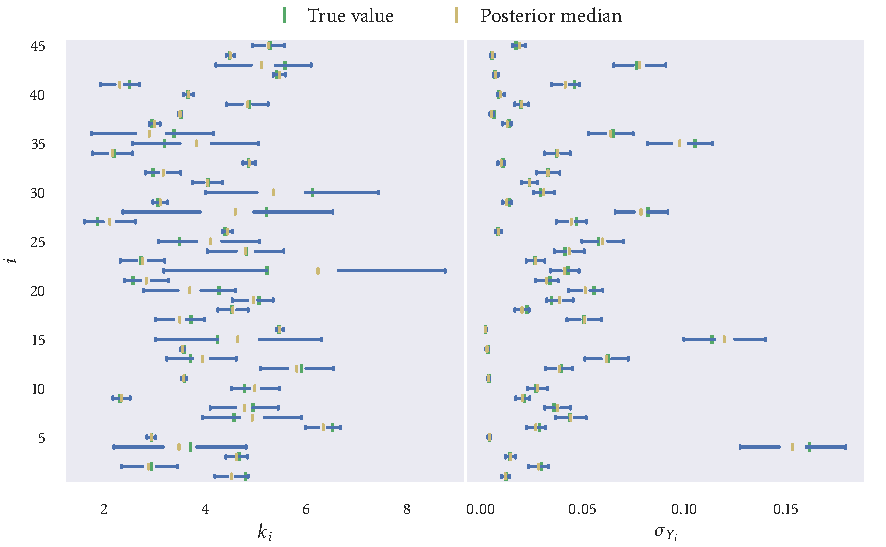
\includegraphics{top/top_hier_summary.pdf}
  \caption{Summarising our posteriors about the interaction and
    noise-scale parameters of the $N=45$ agents simulated according to the
    hierarchical topological model. Box boundaries represent the upper and
    lower quartiles of our beliefs, and the whiskers show the posterior
    median $\pm1.5\times\text{IQR}$.}
  \label{fig:top_hier_summary}
\end{figure}

\section*{Conclusions}

Having shown that we can accurately capture the true parameter values of data
simulated from the hierarchical topological model, we have now demonstrated
that we can perform successful simulation studies on \emph{all} our
\emph{continuous} hierarchical models. In \cref{sec:global_models} we showed
that we can capture the true parameter values of data simulated from our global
models (both and continuous \emph{and} discontinuous).

The inference schemes constructed to perform these inferences can now be
repurposed with minimal-to-no-modification for use with data of real flocking
events. We can be confident in the accuracy and our implementation of these
schemes. With this, if we find our implementations unable to fit real data to
our models, we can be confident that this is due to a discrepancy between model
and data, rather than an error in our implementation.
